%%Berichtvorlage für EDBV WS 2014/2015

\documentclass[paper=A4, deutsch]{scrartcl}
\usepackage[ngerman]{babel}
\usepackage[utf8]{inputenc}
\usepackage{algorithmic}
\usepackage{algorithm}
\usepackage{graphicx}
\usepackage{amsmath,amssymb}
\usepackage{subcaption}
\captionsetup{compatibility=false}
\usepackage{multirow}
\usepackage{color}
\usepackage[]{geometry}
\usepackage{textcomp}

\newcommand\tab[1][1cm]{\hspace*{#1}}

\begin{document}


%%------------------------------------------------------
%% Ab hier tragt ihr eure Daten und Ergebnisse ein:
%%------------------------------------------------------

\title{Lib-Indexer} %%Projekttitel hier eintragen

\subtitle{EDBV WS 2019/2020: AG\_C\_3} %%statt XX Arbeitsgruppenbezeichnung hier eintragen (zB.: A1)


%%Namen und Matrikelnummern der Gruppenmitglieder hier eintragen
\author{Anand Eichner (11808244)\\
Laurenz Edmund Fiala (11807869)\\
Anna Nieto-Berezhinskaya (01223066)\\
Aleksandar Vucenovic (01635282)}



%%------------------------------------------------------

\maketitle


%%------------------------------------------------------
\section{Gewählte Problemstellung}
(1-1,5 Seiten)\\
entspricht dem (aktualisierten) Konzept
\subsection{Ziel}
Das Projekt soll Bücher in einem Bücherregal erkennen, in Bücher-Koordinaten umwandeln und nach ihrem Label abspeichern.

\subsection{Eingabe}
JPG-Bild eines Bücherregals mit Büchern, auf denen eindeutige TU-Bibliotheks-Labels (schwarz-auf-weiß) kleben.

\subsection{Ausgabe}
visuell:\\
\\
\begin{figure}[H]
 \centering
 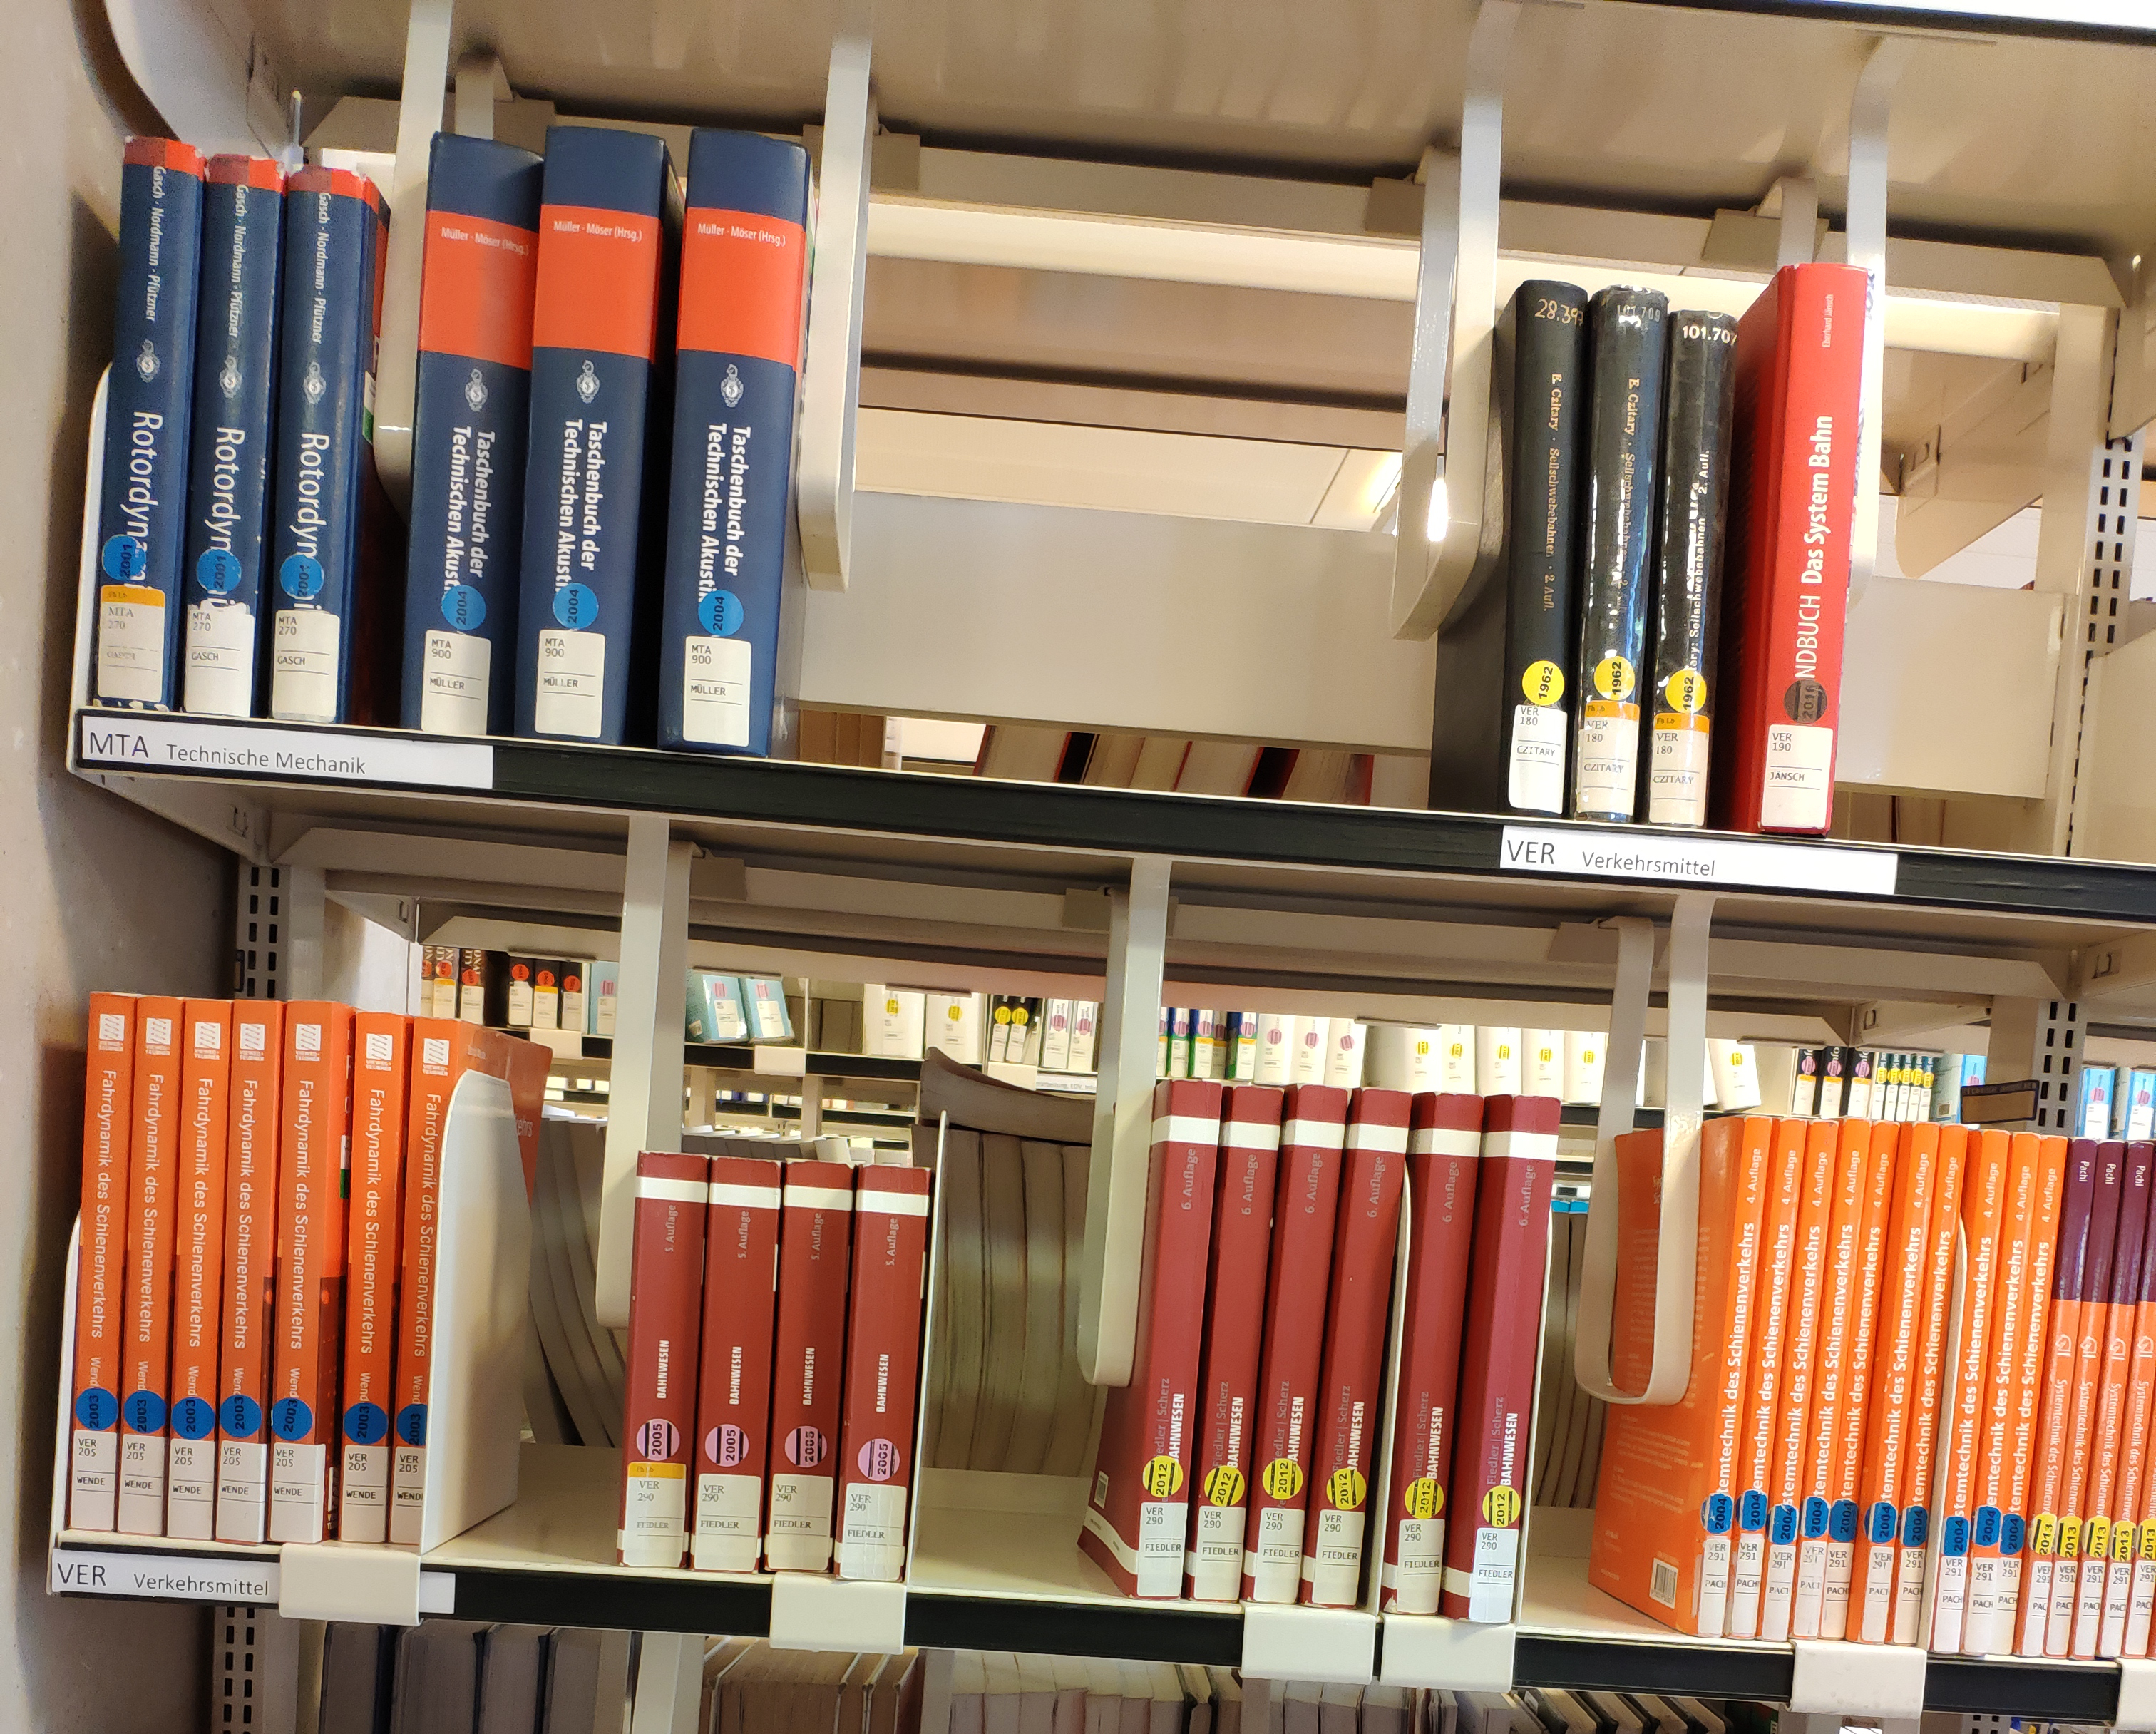
\includegraphics[width=0.4\textwidth]{input.jpg}
 \caption{Input-Bild}
 \label{fig:img}
\end{figure}


\noindent textuell:\\
Strukturierte Klartext-Datei mit Inhalt:
\begin{itemize}
  \item Standort der Bücher (in Büchern zum Ursprung - links-oben)
  \item Vier Pixel-Vektoren, die ein Label in einem Viereck umschließen
\end{itemize}

\subsection{Voraussetzungen und Bedingungen}
\begin{itemize}
  \item Die Bücher müssen gerade (+/- 5°) stehen.
  \item Das Bild darf nicht mehr als 30° von der Waagrechte abweichen.
  \item Das Bild muss eine für die Texterkennung der Labels ausreichende Auflösung aufweisen (Abhängig von der Entfernung).
  \item Das Bild muss farbig sein.
  \item Das Bild muss ausreichend hell sein. 
  \item Ein Weißabgleich muss durchgeführt worden sein.
\end{itemize}

Neue Anforderungen:
\begin{itemize}
  \item Der Hintergrund der Labels muss weiß sein (Intensität muss über dem globalen Otsu-Threshold liegen)
\end{itemize}

\subsection{Methodik}
Methodik- Pipeline
\begin{enumerate}
	\item Hough-Transformation\\
		\textit{Finden der Regalfächer zum Korrigieren der Perspektive}
	\item Persprektivenkorrektur\\tuwe
		\textit{Mittels Transformationsmatrix aus HT berechnet}
	\item Eckenerkennung\\
		\textit{Finden der Ecken von Labels}
	\item Integral imaging\\
		\textit{Finden von Labels innerhalb eines Akzeptanzbereichs, es werden nur Bereiche zwischen verschiedenen, zuvor erkannten, Ecken überprüft}
	\item Eigene Heuristik\\
		\textit{Einordnen von Labels in Buch-Koordinaten}
	\item Optical Character Recognition\\
		\textit{Erkennen von Text auf den Labels in den zuvor erkannten Bereichen}
\end{enumerate}

\subsection{Evaluierungsfragen}
\textbf{Interaktion zwischen den Komponenten:}
\begin{itemize}
	\item \textit{Werden die Regalfächer korrekt erkannt?}\\
		  Voraussetzungen:\tab Seite der Regalfächer, die zur Kamera zeigt, ist schwarz.\\
		  Ergebnis:\tab[2.2cm] An jedem Fach liegt eine Gerade an.
	\item \textit{Wird die Perspektive korrekt angepasst?}\\
		  Voraussetzungen:\tab Korrekte Geraden der Regalfächer.\\
		  Ergebnis:\tab[2.2cm] Bücher und Labels sind im Bild weitestgehend rechteckig.
	\item \textit{Werden alle Labels erkannt?}\\
		  Voraussetzungen:\tab Perspektivenkorrigiertes Bild\\
		  Ergebnis:\tab[2.2cm] Bounding-Boxes der gefundenen Labels
	\item \textit{Sind die Bounding Boxes der gefundenen Labels korrekt? Ist der gesamte Text darin enthalten?}\\
		  Voraussetzungen:\tab Korrekt erkanntes Label oder ein false-positive.\\
		  Ergebnis:\tab[2.2cm] Vier Vektoren, die den gesamten Text umschließen (und nicht mehr). Bei false-positives ist das Ergebnis nicht relevant, jedoch sollte es nicht zu groß sein (z.B. das gesamte Bild überdecken).
	\item \textit{Werden die Labels korrekt in Bücher-Koordinaten umgewandelt?}\\
		  Voraussetzungen:\tab Bounding Boxes der Labels sind korrekt.\\
		  Ergebnis:\tab[2.2cm] Bücher-Koordinatensystem als 2D-Array mit Ursprung links-oben.
	\item \textit{Werden die Labels der TU-Bibliothek korrekt gelesen und in Text umgewandelt?}\\
		  Voraussetzungen:\tab Label Bounding-Boxes wurden korrekt berechnet (enthalten keinen unnötigen Text).\\
		  Ergebnis:\tab[2.2cm] String-Repräsentation des Labels. Erwartete Korrektheit: $>$ 90\% für typische Datensätze.
	\item \textit{Wird die Wahrscheinlichkeit der Label-Korrektheit angemessen berechnet?}\\
		  Voraussetzungen:\tab Korrekt in Text umgewandeltes Label.\\
		  Ergebnis:\tab[2.2cm] Floating-point Wert im Intervall [0, 1]. Alle Labels mit Wahrscheinlichkeit 0 wurden entfernt.
\end{itemize}

\subsection{Zeitplan}
\begin{table}[H]
	\centering
		\begin{tabular}{|c|c|c|}
		\hline
		Meilenstein & abgeschlossen am & Arbeitsaufwand in h\\
		\hline
		Prototyp & 10.11. & 30\\
		\hline
		Hough-Transformation & 17.11. & 50\\
		\hline
		Perspektivenkorrektur & 17.11. & 6\\
		\hline
		Labelerkennung & 25.11. & 80\\
		\hline
		Labels in Buch-Koordinaten & 1.12. & 4\\
		\hline
		Optical Character Recognition & 10.12. & 110\\
		\hline
		Labels filtern & 15.12. & 6\\
		\hline
		Daten in Output-Format umwandeln & 15.12. & 4\\
		\hline
		Tests & 18.12. & 5\\
		\hline
		Evaluierung & 20.12. & 5 \\
		\hline
		\end{tabular}
\end{table}
%%------------------------------------------------------

%%------------------------------------------------------
\section{Arbeitsteilung}
\begin{center}
  \begin{tabular}{ |l | c | }
    \hline
  Name & Tätigkeiten\\
    \hline
    	Anna Nieto-Berezhinskaya & ?\\
		\hline
		Anand Eichner & houghTransform (+ locals), PerspectiveCorrection (+ locals),\\
		\hline
		Laurenz Edmund Fiala & label\_detection (+ locals),\\
		\hline
		Aleksandar Vucenovic & ocr (+ locals), ncc, ssd\_naive (+ locals),\\
		 & preprocessing (+ locals)\\
		\hline
  \end{tabular}
\end{center}

%%------------------------------------------------------

%%------------------------------------------------------
\section{Methodik}
(2-3 Seiten)\\
Hier wird die verwendete Methodik in der Theorie vorgestellt:\\
Welche Methodik wurde verwendet? Warum eignet sich diese Methodik für die gewählte Problemstellung? Habt ihr Methoden verändert (Einschränkungen, Abwandlungen, Parameter), wenn ja wie? etc.\\
Die erwähnten Methoden werden zum größten Teil auf Beschreibungen in Büchern oder wissenschaftlichen Artikeln beruhen. Daher ist hier auch der richtige Platz für Zitate. Die hier zitierten Publikationen sollten mittels Abkürzung bzw. Nummer referenziert sein und sich in der Referenzliste am Ende des Berichts über diese Bezeichnung finden lassen.\\
Ein Beispielsatz (inkl. entsprechender Literaturangabe am Ende des Berichts): Interest Points wurden mittels Scale Invariant Feature Transform \cite{lowe2004} detektiert.\\
Bei der Verwendung von Latex gestaltet sich das Zitieren besonders einfach - siehe Beispielssatz im Source der Latex-Vorlage.\\
\textbf{Wichtig in diesem Abschnitt ist, dass sich der Leser Eures Berichts mit den verwendeten Methodiken auskennt und weiß, weshalb ihr diese Methodiken verwendet habt und keine anderen. Es soll dem Leser helfen den nächsten Abschnitt des Berichts besser zu verstehen.}
%%------------------------------------------------------

%%------------------------------------------------------
\section{Implementierung}
(1-X Seiten)\\
Hier gebt ihr einen Überblick über Eure Implementierung:\\
Wie habt ihr die im vorhergehenden Abschnitt vorgestellte Methodik praktisch umgesetzt? Wie werden die einzelnen Methoden kombiniert (zB. Implementierungspipeline)?\\
Hier ist Platz für Implementierungsdetails wie zB. gewählte Parameter. \\
Wie startet der User das Programm? Welche Parameter hat der User zu setzen?\\
Auch in diesem Abschnitt können Referenzen und Zitate notwendig sein.\\
\textbf{Wichtig in diesem Abschnitt ist, dass der Leser Eures Berichts versteht wie ihr Euer Projekt in MATLAB umgesetzt habt um sich auch im Quelltext leichter zurechtfinden zu können.}
%%------------------------------------------------------

%%------------------------------------------------------
\section{Evaluierung}
(2-X Seiten)\\
Hier stellt ihr Euren Datensatz vor und beantwortet Evaluierungsfragen:\\
z.B. Fakten zum Datensatz: Anzahl der Bilder, Größe der Bilder, Quelle des Datensatzes (falls selbst aufgenommen: Aufnahmegerät, Einstellungen,... / falls nicht selbst erstellt: Datenbank vorstellen... $\to$ Referenzen!)\\
Diskussion der Evaluierungsfragen: Beantwortung der Fragen, Diskussion anhand von Beispielen, Diskussion von Grenzfällen: für welche Bilder funktioniert die Implementierung, für welche nicht? Worin unterscheiden sich diese Bilder? Warum funktionieren sie nicht? etc.\\
Evaluiert wird der ganze Datensatz, nicht nur einzelne Bilder. Einzelne Bilder können zum Aufzeigen von Fehlern/Problemen/besonders guten Ergebnissen... genutzt werden.\\
Zur Evaluierung gehört auch das Testen der einzelnen Methodiken (separat), mit Erwähnung eventueller Einschränkungen.
%%------------------------------------------------------

%%------------------------------------------------------
\section{Schlusswort}
(max. 1 Seite)\\
Hier fasst ihr Ergebnisse Eures Projekt zusammen:\\
Welche Schlussfolgerung lässt sich ziehen? Gibt es offene Probleme? Wie lässt sich Eure Lösung noch verbessern? etc.
%%------------------------------------------------------

%%------------------------------------------------------
\bibliographystyle{plain}
\bibliography{edbv_lit}
%%Bei verwendung von Latex schreibt ihr eure Referenzen in ein eigenes bib-File (siehe hier edbv_lit.bib). Jene Referenzen, die ihr im Bericht mittels \cite zitiert, werden automatisch in die Referenzliste übernommen. Weitere Information zum Einbinden von BibTex gibt es hier: http://www.bibtex.org/Using/de/
%%------------------------------------------------------
\textbf{Webseiten werden als Fußzeilen (an jener Stelle wo sie verwendet werden) eingebunden, nicht als Literature!}

\end{document}
\grid
\grid
